\chapter{Background Modeling}
\label{chap:modeling}

The study dedicated to the modeling of the major background is shown in this chapter.
The V+jets, which is the dominant background in all three lepton channels, has a known issue of mismodeling. 
The reweighting is applied to the V+jet background sample, as described in the following sections.
Details are shown in the 2-lepton channel for Z+jets sample. 
In the 1-lepton channel, a similar procedure is applied to the W+jets sample, and in the 0-lepton channel reweighting is applied for the sum of Z+jets sample and W+jets sample.

\section{$m_{jj}^{tag}$ reweighting}
Figure~\ref{fig:2lep_mtag_before_rw} shows the $m^{tag}_{jj}$ distributions in CR of merged and resolved selection in the 2-lepton channel.

\begin{figure}[ht]
    \centering
    \includegraphics[width=0.48\textwidth]{figures/2lep/reweighting/before_reweighting/C_0ptag1pfat0pjet_0ptv_CRVjet_MTagMerJets_Log.eps}
    \includegraphics[width=0.48\textwidth]{figures/2lep/reweighting/before_reweighting/C_0ptag2pjet_0ptv_CRVjet_Fid_MTagResJets_Log.eps}
    \caption{ $m^{tag}_{jj}$ distributions before applying reweighting for the merged (left) and resolved (right) control regions in the 2-lepton channel.}
    \label{fig:2lep_mtag_before_rw}
\end{figure}

The mismodelling is observed as a slope in the ratio of data/MC in both regions.
These discrepancies have been known in the previous analysis round~\cite{STDM-2017-20}, as well as in other ATLAS analyses. 
This effect is believed to be due to the tuning of the QCD parameters, related to the combination of the shower activity and the scale choice for NLO real emissions in Sherpa~2.2.1.
The discrepancies are also seen with other kinematics mainly related to the jets other than signal jets. The distribution of the number of small-R jets and the $p_\mathrm{T}$ of the two forward jets, and the RNN score are shown in figure~\ref{fig:before_rw}, showing discrepancies as slopes between data and MC.
\begin{figure}[ht]
    \centering
    \includegraphics[width=0.48\textwidth]{figures/2lep/reweighting/before_reweighting/C_0ptag1pfat0pjet_0ptv_CRVjet_NJets_Lin.eps}
    \includegraphics[width=0.48\textwidth]{figures/2lep/reweighting/before_reweighting/C_0ptag2pjet_0ptv_CRVjet_Fid_NJets_Lin.eps}
    \includegraphics[width=0.48\textwidth]{figures/2lep/reweighting/before_reweighting/C_0ptag1pfat0pjet_0ptv_CRVjet_PtTagMerJets_Log.eps}
    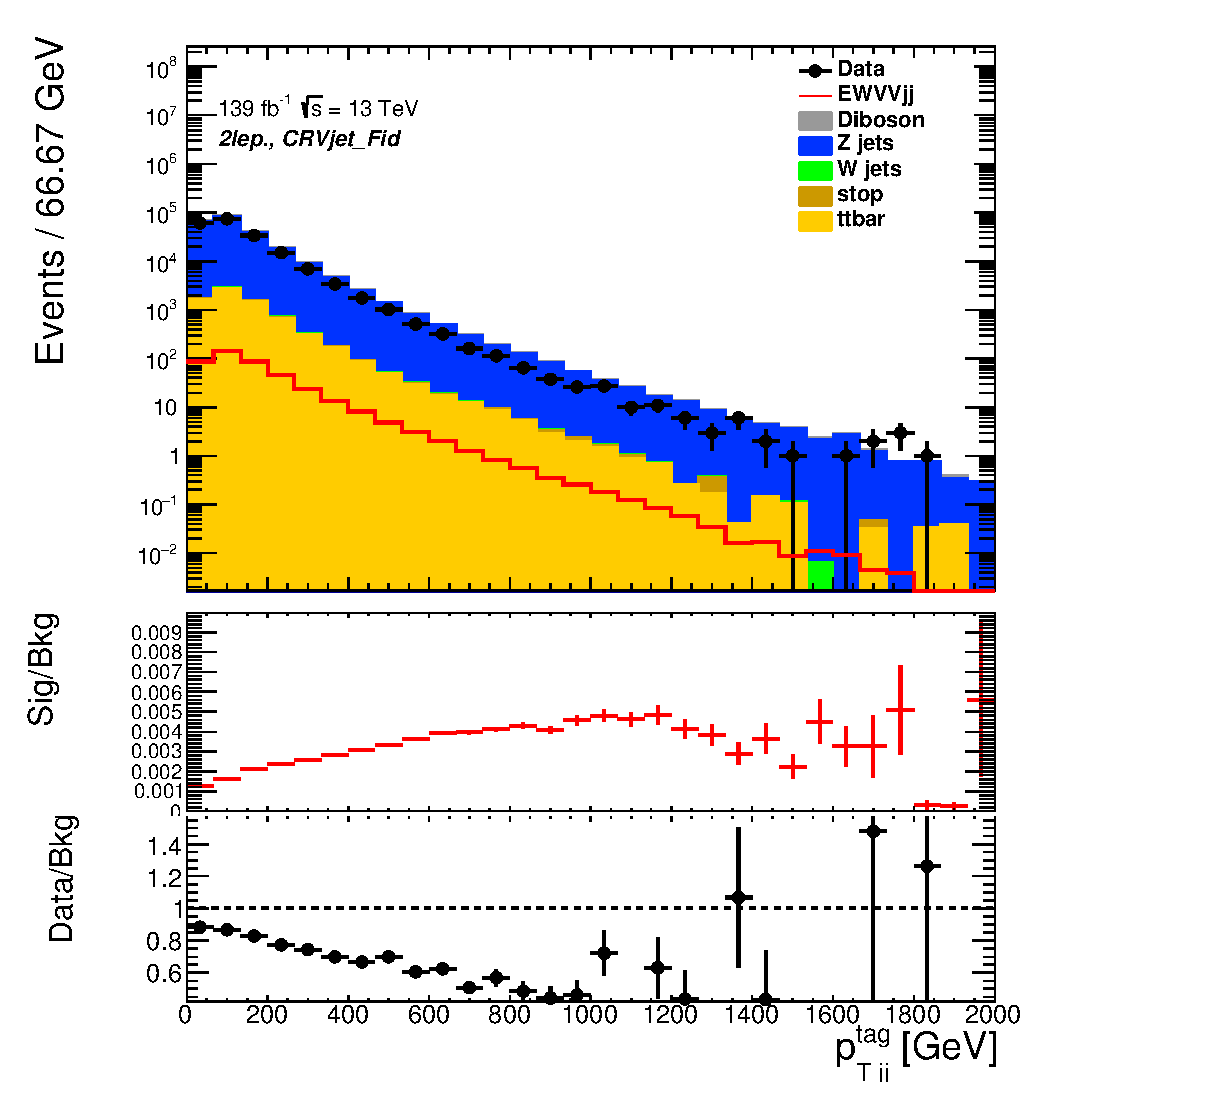
\includegraphics[width=0.48\textwidth]{figures/2lep/reweighting/before_reweighting/C_0ptag2pjet_0ptv_CRVjet_Fid_PtTagResJets_Log.eps}
    \includegraphics[width=0.48\textwidth]{figures/2lep/reweighting/before_reweighting/C_0ptag1pfat0pjet_0ptv_CRVjet_RNNScoreMerged_Lin.eps}
    \includegraphics[width=0.48\textwidth]{figures/2lep/reweighting/before_reweighting/C_0ptag2pjet_0ptv_CRVjet_Fid_RNNScoreResolved_Lin.eps}
    \caption{ Distributions of number of jets and the $p_\mathrm{T}$ of the two forward jets, and RNN score before applying reweighting for the merged (left) and resolved (right) control regions in the 2-lepton channel.}
    \label{fig:before_rw}
\end{figure}

The reweighting is applied to the V+jets background sample to partly compensate for this mismodeling before defining the SRs and CRs. 
The data/MC ratio is parameterized by the simple linear function and the estimated reweighting factor is applied by the event-by-event weight. 
%A simple linear fit is performed to the ratio between V+jets MC and the observed data in $m^{tag}_{jj}$ distribution, in each V+jets CRs. 
The fit function is defined as:
\begin{equation}
\label{eqn:reweight}
R=p_{0} * m_{jj}^{tag}+p_{1}
\end{equation}
where the $R$ is defined as the ratio of data over V+jets MC in each bin.
The fitting and the correction is performed only for the V+jets samples, therefore contributions of other MC samples are subtracted from data at first. 
Inclusive MC samples corresponding to the full Run-2 dataset are used for deriving the reweighting function, since the fitted value did not depend on the pile-ups.
In figure~\ref{fig:LinearFit}, the fitted line as a function of $m^{tag}_{jj}$ is shown. 

\begin{figure}[ht]
    \centering
    \includegraphics[width=0.40\textwidth]{figures/2lep/reweighting/MTagMerJets_0ptag1pfat0pjet_0ptv_CRVjet_finerbin}
    \includegraphics[width=0.40\textwidth]{figures/2lep/reweighting/MTagResJets_0ptag2pjet_0ptv_CRVjet_Fid_finerbin}
    \caption{ Fitted slope in data/MC ratio of $m^{tag}_{jj}$ distributions, in merged CR (left) and resolved CR (right). The dotted line shows the 1~$\sigma$ error of the fitting result of the linear function. }
    \label{fig:LinearFit}
\end{figure}

Both distributions of the V+jets MC are first normalized to the data then the correction function (\ref{eqn:reweight}) is derived. 
The binning is done in such a way that each bin contains at least 100 Z+jets events in order to have less than 10~\% statistical uncertainty. 
In merged control region, due to the large statistic difference between the low-mass region and the high-mass region, the barycenter of each bin is used as a fitting point, while in resolved control region the bin center is used.
The estimated reweighting factor is applied as an event-by-event weight, also in the signal region.
The fitted parameter is summarized in the table~\ref{tab:fit}. 
\begin{table}[htbp]
 \footnotesize
\begin{center}
\begin{tabular}{ | c | c | c |}
\hline
Parameter & Merged CRVjet & Resolved CRVjet  \\
\hline
$p_{0}$ (slope) [$\GeV^{-1}$] & $(30.2 \pm 3.1)~e^{-5}$ &  $(-17.5 \pm 0.5)~e^{-5}$ \\
 \hline
$p_{1}$ (constant)  & $1.362 \pm 0.032$ & $1.187 \pm 0.005$ \\
\hline
\end{tabular}
\caption{\label{tab:fit} Fitted re-weighting parameters for the merged and resolved regions of the 2-lepton channel. The errors written here are the uncertainties of the fitted parameters. }
  \end{center}
\end{table}
The reweighted distributions are shown in Figure~\ref{fig:2lep_mtag_after_rw}. 
The data/MC ratios are more flat compared to the figure~\ref{fig:2lep_mtag_before_rw}, indicating successful reweighting.
Only the difference of the shape is corrected by this reweighting procedure as seen in the data/MC ratio around 0.8. 
The difference in the normalization is accounted for in the final fitting.
In the resolved CR, there is still a discrepancy above 2500~GeV since it seems the linear function is not enough to model the mismodelling in this CR.
The uncertainty on the reweighting factor is conservatively assigned in the final fitting setup, which is going to be explained in chapter~\ref{chap:systematics}.
\begin{figure}[ht]
    \centering
    \includegraphics[width=0.48\textwidth]{figures/2lep/reweighting/after_reweighting/C_0ptag1pfat0pjet_0ptv_CRVjet_MTagMerJets_Log.eps}
    \includegraphics[width=0.48\textwidth]{figures/2lep/reweighting/after_reweighting/C_0ptag2pjet_0ptv_CRVjet_Fid_MTagResJets_Log.eps}
    \caption{ $m^{tag}_{jj}$ distributions after applying reweighting for the merged (left) and resolved (right) control regions in the 2-lepton channel. The slope seen before reweighting is corrected in the Z+jet CR.}
    \label{fig:2lep_mtag_after_rw}
\end{figure}

The comparison of distributions of data and MC for the number of small-R jets and $p_\mathrm{T}$ of the two forward jets, and the RNN score after reweighting are shown in Figure \ref{fig:after_rw}
respectively. The discrepancy is relaxed by the reweighting procedure, while it is not fully corrected especially for the $p_\mathrm{T}$ of the two forward jets.
The RNN score distribution is also corrected since it learns the high-level information like $m^{tag}_{jj}$.
The RNN score still has the discrepancy in the normalization as well as its shape, which can be seen as a slope especially in the merged CR.
Those discrepancy will be corrected by the final fitting described in chapter~\ref{chap:statistics}.
\begin{figure}[ht]
    \centering
    \includegraphics[width=0.48\textwidth]{figures/2lep/reweighting/after_reweighting/C_0ptag1pfat0pjet_0ptv_CRVjet_NJets_Lin.eps}
    \includegraphics[width=0.48\textwidth]{figures/2lep/reweighting/after_reweighting/C_0ptag2pjet_0ptv_CRVjet_Fid_NJets_Lin.eps}
    \includegraphics[width=0.48\textwidth]{figures/2lep/reweighting/after_reweighting/C_0ptag1pfat0pjet_0ptv_CRVjet_PtTagMerJets_Log.eps}
    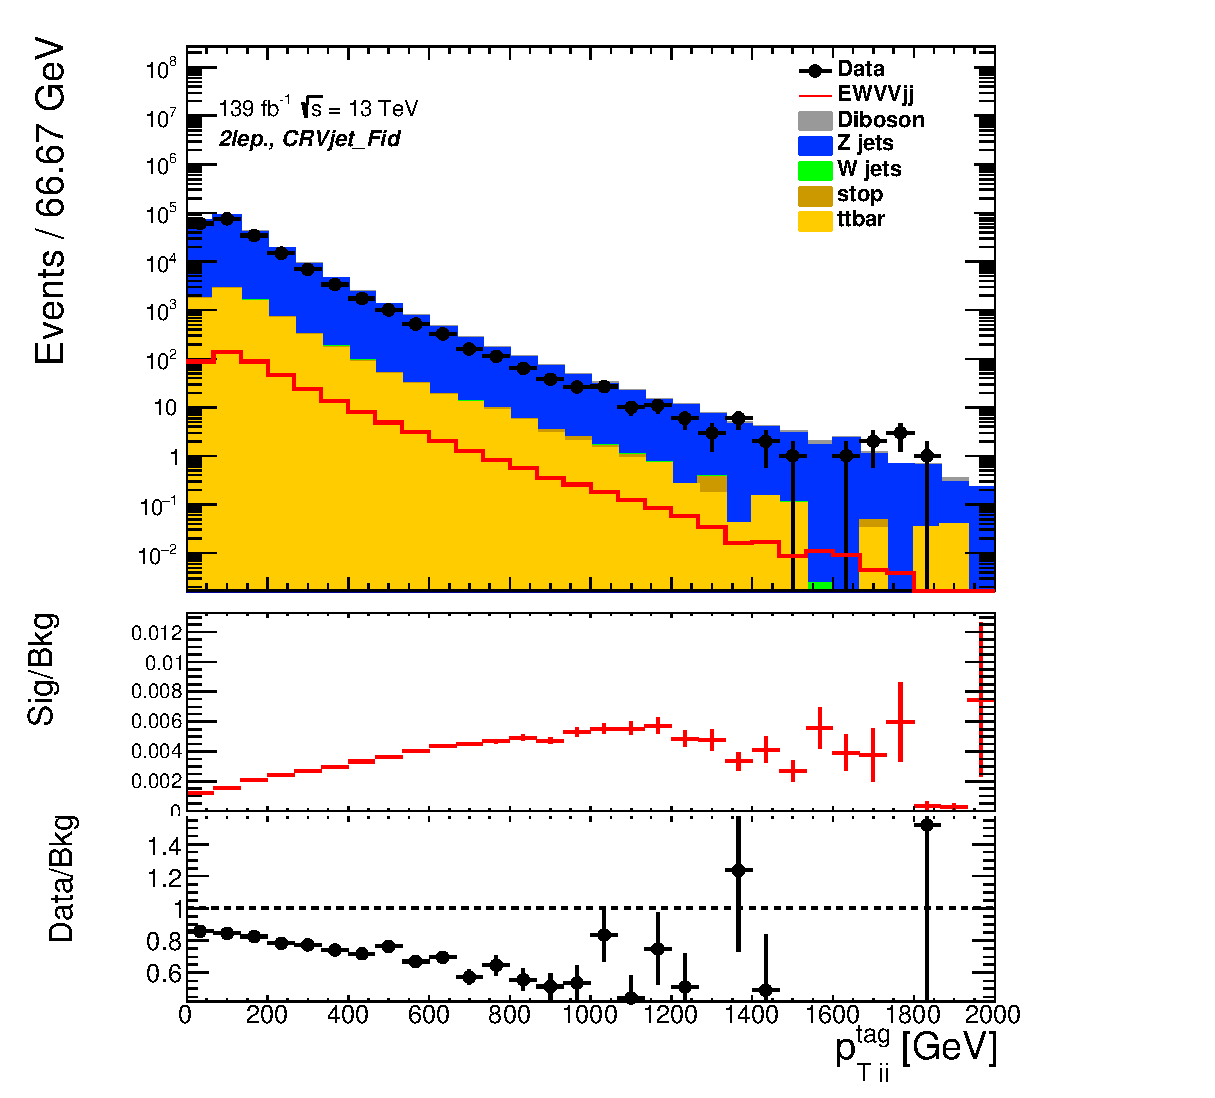
\includegraphics[width=0.48\textwidth]{figures/2lep/reweighting/after_reweighting/C_0ptag2pjet_0ptv_CRVjet_Fid_PtTagResJets_Log.eps}
    \includegraphics[width=0.48\textwidth]{figures/2lep/reweighting/after_reweighting/C_0ptag1pfat0pjet_0ptv_CRVjet_RNNScoreMerged_Lin.eps}
    \includegraphics[width=0.48\textwidth]{figures/2lep/reweighting/after_reweighting/C_0ptag2pjet_0ptv_CRVjet_Fid_RNNScoreResolved_Lin.eps}
    \caption{ Distributions of the number of jets and the $p_\mathrm{T}$ of the two forward jets after applying reweighting for the merged (left) and resolved (right) control regions in the 2-lepton channel.}
    \label{fig:after_rw}
\end{figure}
% njets and pt plots after reweighting
% 2-lepton new merged CR - plots
%\begin{figure}[ht]
% \centering
%   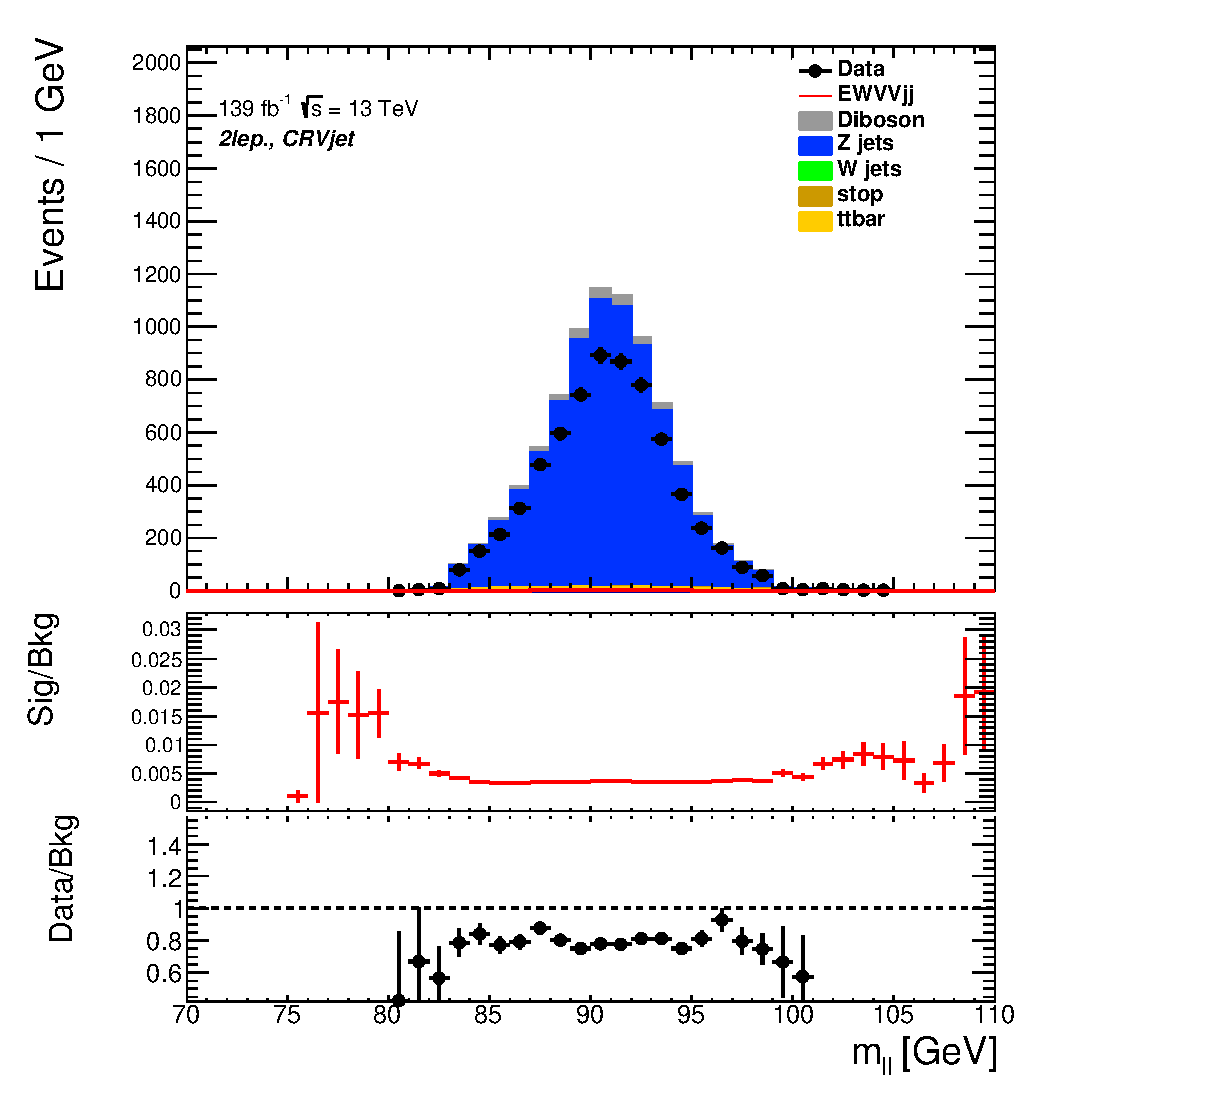
\includegraphics[width=0.48\textwidth]{figures/2lep/reweighting/after_reweighting/C_0ptag1pfat0pjet_0ptv_CRVjet_llMass_Lin.eps}
%   \includegraphics[width=0.48\textwidth]{figures/2lep/reweighting/after_reweighting/C_0ptag1pfat0pjet_0ptv_CRVjet_MllJ_Lin.eps}
%   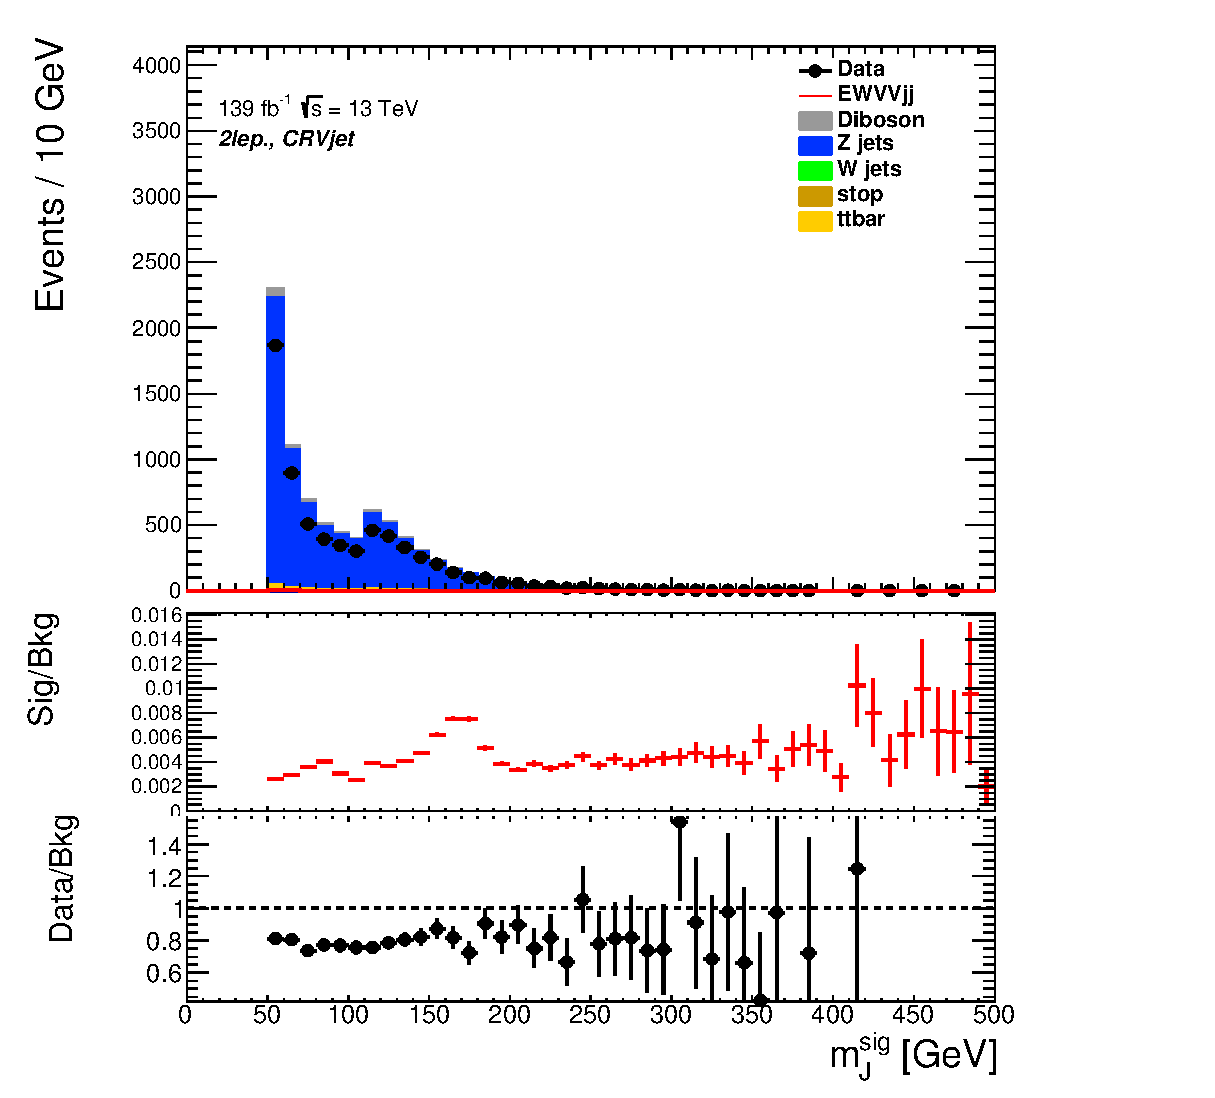
\includegraphics[width=0.48\textwidth]{figures/2lep/reweighting/after_reweighting/C_0ptag1pfat0pjet_0ptv_CRVjet_fatJetMass_Lin.eps} \\
%
%   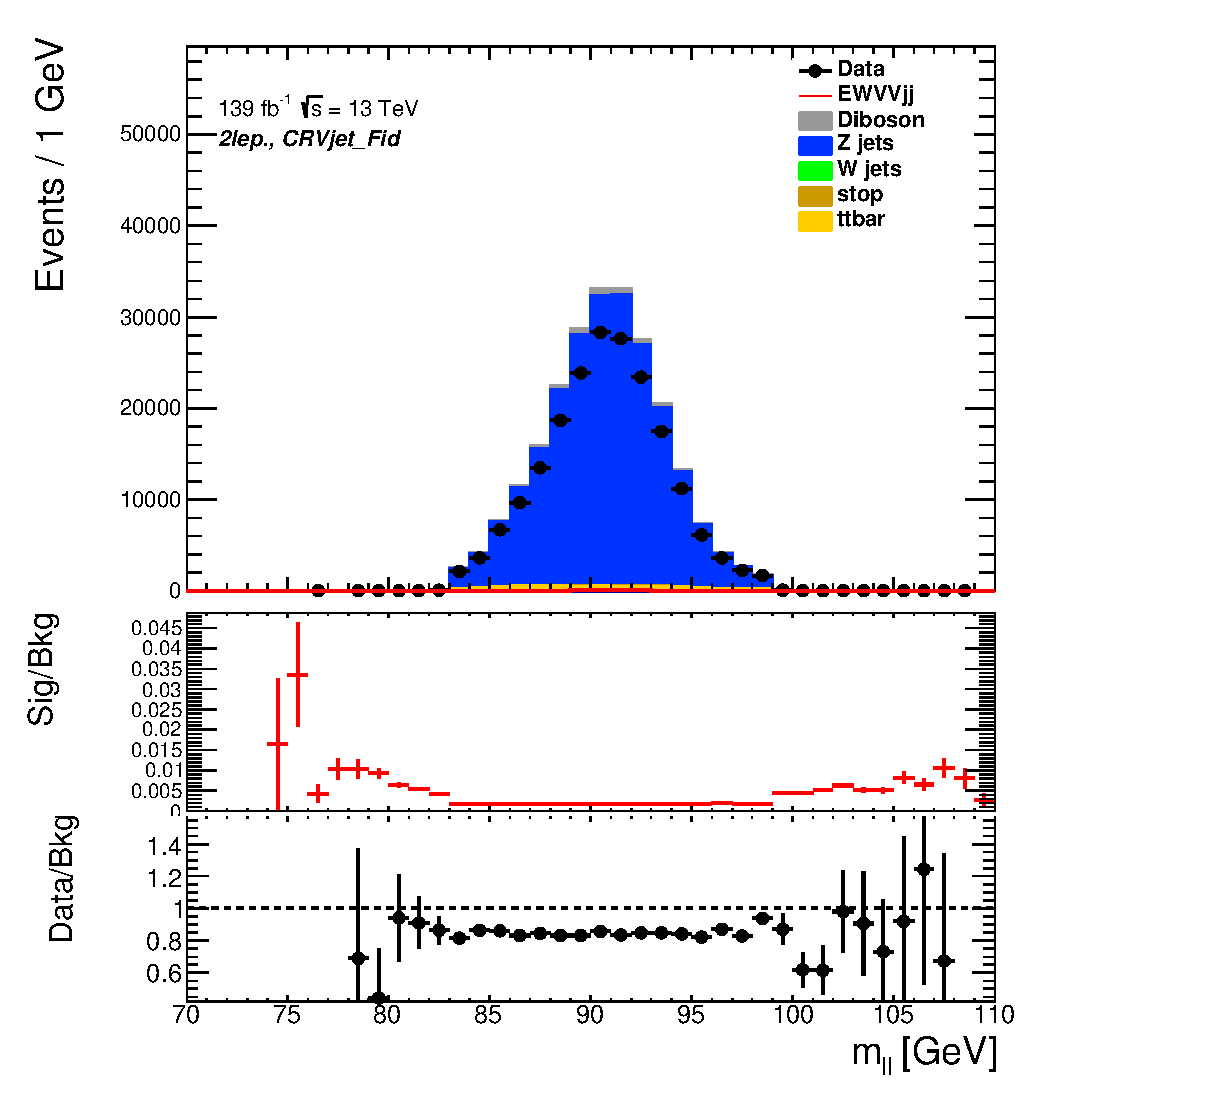
\includegraphics[width=0.48\textwidth]{figures/2lep/reweighting/after_reweighting/C_0ptag2pjet_0ptv_CRVjet_Fid_llMass_Lin.eps}
%   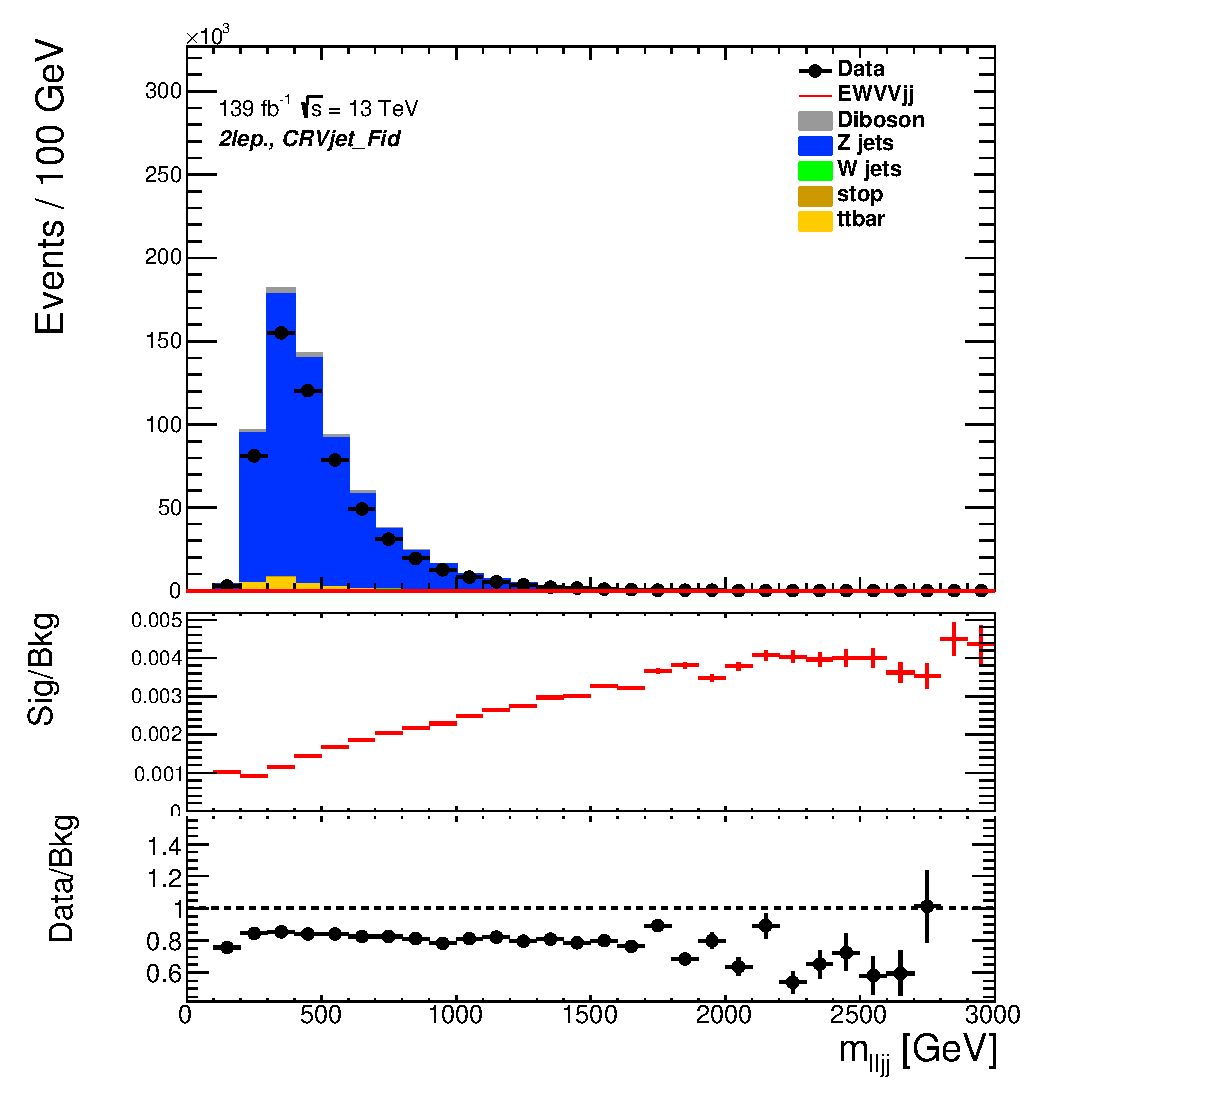
\includegraphics[width=0.48\textwidth]{figures/2lep/reweighting/after_reweighting/C_0ptag2pjet_0ptv_CRVjet_Fid_Mlljj_Lin.eps}
%  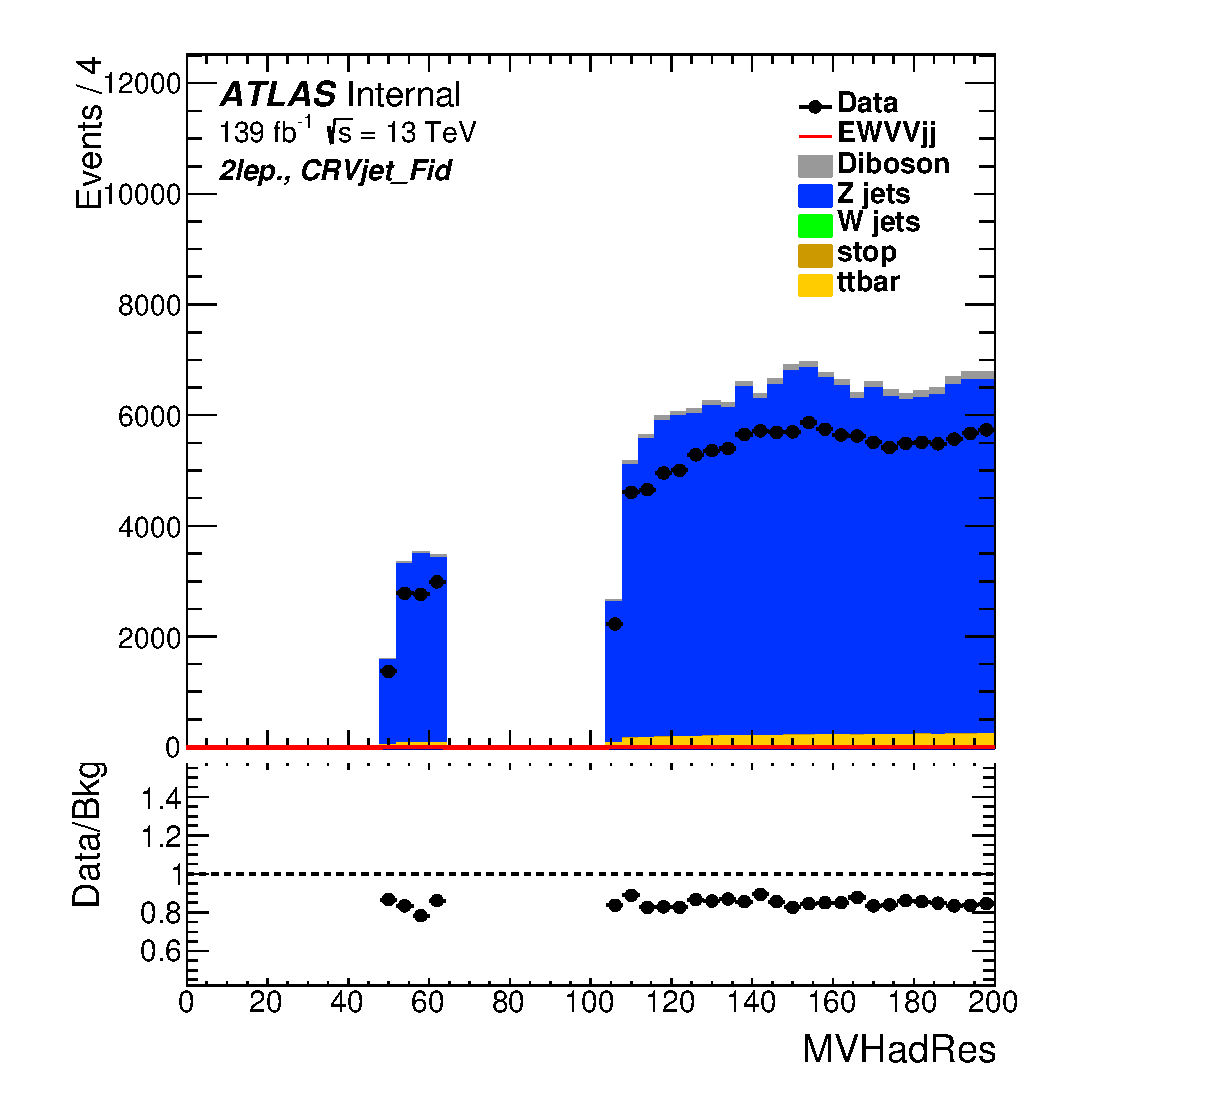
\includegraphics[width=0.48\textwidth]{figures/2lep/reweighting/after_reweighting/C_0ptag2pjet_0ptv_CRVjet_Fid_MVHadRes_Lin.eps}
%  \caption{ Various kinematic variables in the Z+jets merged CR (up), and Z+jets resolved (below) in the 2-lepton channel analysis.}
%   \label{fig:2lep_zjets_resolved_CR}
%\end{figure}

%************write something about MadGraph and the dedicated modeling uncertainty here**********
There is alternative samples using MadGraph instead of Sherpa~2.2.1 as a generator. 
The modeling of the MadGraph in 2-lepton Z+jets CRs is shown in figure~\ref{fig:SherpaMadGraph}. 
No reweighting is applied in figure~\ref{fig:SherpaMadGraph} for comparison. 
Backgrounds are normalized to the data to see the shapes of the MC. 
MadGraph has better modeling in our phase space including the high $m^{tag}_{jj}$ region. 
However, Sherpa is used as the baseline sample since the sample with larger statistics was available.
This difference between the two generators is included in the final fitting as a theoretical uncertainty, described in detail in chapter~\ref{chap:systematics}.
\begin{figure}[ht]
    \centering
    \includegraphics[width=0.49\textwidth]{figures/2lep/reweighting/MTagResJets_0ptag2pjet_0ptv_CRVjet_ratio.pdf}
    \includegraphics[width=0.49\textwidth]{figures/2lep/reweighting/MTagMerJets_0ptag1pfat0pjet_0ptv_CRVjet_ratio.pdf}
    \caption{ $m^{tag}_{jj}$ distributions before applying reweighting for Sherpa~2.2.1 (red) and MadGraph (blue). Sherpa~2.2.11 (green), the newly modified version is also compared, showing that there is little improvement in slope compared to MadGraph.}
    \label{fig:SherpaMadGraph}
\end{figure}


